\documentclass[11pt]{article}

\usepackage[margin=1in]{geometry}
\usepackage{amsmath, amssymb, amsthm}
\usepackage{array}
\usepackage{booktabs}
\usepackage{enumitem}
\usepackage{graphicx}
\usepackage{hyperref}
\usepackage{pgfplots}
\usepackage[most]{tcolorbox}
\usepackage[table]{xcolor}
\usepackage{tikz}
\usetikzlibrary{arrows.meta,fit,positioning}
\pgfplotsset{compat=1.18}

\newcolumntype{L}[1]{>{\raggedright\arraybackslash}p{#1}}
\newcommand{\calendarentry}[1]{\rule{0pt}{2.9ex}#1}
\definecolor{SoftBlue}{HTML}{EEF6FC}
\definecolor{FrameBlue}{HTML}{2C6E91}
\definecolor{SoftGold}{HTML}{FFF4E5}
\definecolor{FrameGold}{HTML}{A55F00}
\definecolor{SoftGreen}{HTML}{EAF7ED}
\definecolor{FrameGreen}{HTML}{2E7D32}

\setlength{\parindent}{0pt}
\setlength{\parskip}{0.45em}
\setlist[itemize]{leftmargin=1.6em,labelsep=0.55em,itemsep=0.2em,topsep=0.3em,parsep=0pt,partopsep=0pt}
\setlist[enumerate]{leftmargin=1.8em,labelsep=0.5em,itemsep=0.2em,topsep=0.3em,parsep=0pt,partopsep=0pt}

\newtcolorbox{examplebox}[1][]{
    enhanced,
    breakable,
    colback=SoftBlue,
    colframe=FrameBlue,
    boxrule=0.9pt,
    arc=2pt,
    left=8pt,
    right=8pt,
    top=6pt,
    bottom=6pt,
    fonttitle=\bfseries,
    #1
}

\newtcolorbox{keybox}[1][]{
    enhanced,
    breakable,
    colback=SoftGold,
    colframe=FrameGold,
    boxrule=0.9pt,
    arc=2pt,
    left=8pt,
    right=8pt,
    top=6pt,
    bottom=6pt,
    fonttitle=\bfseries,
    #1
}

\newtcolorbox{reviewbox}[1][]{
    enhanced,
    breakable,
    colback=SoftGreen,
    colframe=FrameGreen,
    boxrule=0.9pt,
    arc=2pt,
    left=8pt,
    right=8pt,
    top=6pt,
    bottom=6pt,
    fonttitle=\bfseries,
    #1
}

\title{Class 1 Reserved-Slot Strategies: Day-Level Formulation}
\author{Alexandre SEPULVEDA de DIETRICH\\Under the supervision of Pr.~Carri Chan}
\date{\today}

\begin{document}
\maketitle
\setcounter{tocdepth}{3}
\tableofcontents
\bigskip

\section{Introduction}

\subsection{Purpose and Reader Map}

This note is a companion to \texttt{first\_two\_class\_simulation\_note\_v2.tex}. It keeps the same
day-level notation, the same patient behavior objects, and the same metric interpretation, but it
adds a strict booking strategy in which Class 1 has protected daily capacity.

\begin{keybox}[title={Core Policy Question}]
The pooled FCFS baseline asks which patient arrives first. The reserved-slot strategy asks whether
some daily capacity should be protected for Class 1 before the two classes compete for the remaining
slots.
\end{keybox}

The two strategies compared in this note are:
\begin{itemize}[nosep]
    \item \textbf{Pooled FCFS:} every class competes for the same \(S\) daily slots.
    \item \textbf{Strict Class 1 reservation:} \(Q=10\) slots per day are reserved for Class 1 only; unused reserved slots stay empty.
\end{itemize}

\begin{keybox}[title={Future Focus: Soft Reservation}]
A soft reservation or Class-1-priority backfill policy remains a possible future extension. It is not
part of the current code or notebook exploration.
\end{keybox}

\subsubsection{What Changes from the FCFS Note}

\begin{center}
\small
\begin{tabular}{L{0.27\textwidth} L{0.30\textwidth} L{0.33\textwidth}}
\toprule
\textbf{Object} & \textbf{FCFS baseline} & \textbf{Reserved-slot replacement} \\
\midrule
Daily capacity & one pooled capacity \(S\) & protected capacity \(Q\) plus general capacity \(S-Q\) \\
\addlinespace
Calendar state & \(X_{i,r}^{D}\), \(N_r^D\) & same \(X_{i,r}^{D}\), plus audit-layer pool counts \(X_{i,r,\mathrm{res}}^{D}\) and \(X_{i,r,\mathrm{gen}}^{D}\) \\
\addlinespace
Offer rule & earliest residual day with \(N_r^D<S\) & earliest residual day with eligible pool capacity \\
\addlinespace
No-offer logic & no pooled slot is available & no eligible pool is available for that class and policy \\
\addlinespace
Service, cancellation, no-show & unchanged & unchanged \\
\bottomrule
\end{tabular}
\normalsize
\end{center}

\section{Model Formulation}

\subsection{Notation Inherited from v2}

The simulation clock is still the day \(D\). The basic objects are unchanged:
\begin{itemize}[nosep]
    \item \(S\): total appointment slots available per day.
    \item \(H\): rolling booking horizon in days.
    \item \(\mathcal I=\{1,2\}\): patient classes.
    \item \(r\in\{0,1,\dots,H-1\}\): residual delay, where \(r=0\) means appointments scheduled for today.
    \item \(\tau\): original offered delay accepted by a booked patient.
    \item \(X_{i,r}^{D}\): number of class-\(i\) patients scheduled for day \(D+r\).
    \item \(N_r^D=\sum_{i\in\mathcal I}X_{i,r}^{D}\): total scheduled patients on residual day \(r\).
\end{itemize}

The same residual-delay/original-delay distinction remains:
\begin{keybox}[title={Residual Delay vs. Original Delay}]
Residual delay \(r\) is part of the rolling calendar state and decreases when the day advances.
Original delay \(\tau\) is stored with the booking because balking and no-show behavior use the delay
the patient was originally offered.
\end{keybox}

To make the policy formulas match the current implementation and remain compatible with the v2
notation, define the bookable residual-day set
\[
\mathcal R\subseteq\{0,1,\dots,H-1\}.
\]
In the current Python engine, same-day booking is allowed, so
\[
\mathcal R=\{0,1,\dots,H-1\}.
\]
If a future-only convention is desired, the same formulas apply after replacing \(\mathcal R\) with
\(\{1,\dots,H-1\}\).

\subsection{Reservation Parameters}

Let the protected class be
\[
i^\star=1,
\]
and let
\[
Q=10
\]
be the number of Class 1 reserved slots per day. Since the baseline capacity is \(S=32\), the general
pool has
\[
S-Q=22
\]
slots per day.

The total day-level state \(X_{i,r}^{D}\) is still the main state, but the reserved policies require
an audit-layer pool label. Write
\[
X_{i,r,\mathrm{res}}^{D}
=
\text{number of class-}i\text{ patients scheduled in reserved slots on day }D+r,
\]
and
\[
X_{i,r,\mathrm{gen}}^{D}
=
\text{number of class-}i\text{ patients scheduled in general slots on day }D+r.
\]
Then
\[
X_{i,r}^{D}
=
X_{i,r,\mathrm{res}}^{D}
+
X_{i,r,\mathrm{gen}}^{D}.
\]

Define the pool occupancies
\[
R_r^D=\sum_{i\in\mathcal I}X_{i,r,\mathrm{res}}^{D},
\qquad
G_r^D=\sum_{i\in\mathcal I}X_{i,r,\mathrm{gen}}^{D},
\]
so that
\[
N_r^D=R_r^D+G_r^D.
\]

The capacity constraints are
\[
R_r^D\le Q,
\qquad
G_r^D\le S-Q,
\qquad
N_r^D\le S.
\]

\begin{examplebox}[title={Daily Capacity Split for the Implemented Strategy}]
\begin{center}
\small
\renewcommand{\arraystretch}{1.35}
\begin{tabular}{L{0.24\textwidth} L{0.22\textwidth} L{0.42\textwidth}}
\toprule
\textbf{Pool} & \textbf{Capacity} & \textbf{Eligibility} \\
\midrule
Reserved pool & \(Q=10\) & Class 1 only \\
\addlinespace
General pool & \(S-Q=22\) & Class 1 overflow and Class 2 \\
\addlinespace
Total day & \(S=32\) & all scheduled patients, regardless of pool label \\
\bottomrule
\end{tabular}
\normalsize
\end{center}
\end{examplebox}

\subsection{Patient Behavior is Unchanged}

The class behavior object remains
\[
C_i=\{\lambda_i,b_i(\tau),\phi_i,\xi_i(\tau)\}.
\]
The reservation policy does not change arrival rates, balking, cancellation, or no-show behavior.
They only change which residual day and which capacity pool an arriving patient is offered.

\begin{keybox}[title={What the Reservation Strategy Does Not Change}]
For a class-\(i\) patient offered delay \(\tau\), the balking probability remains \(b_i(\tau)\).
For a booked class-\(i\) patient scheduled in the future, the daily cancellation probability remains
\(\phi_i\). At service time, the no-show probability remains \(\xi_i(\tau)\).
\end{keybox}

\section{Booking Rules}

\subsection{Pooled FCFS Baseline}

The pooled FCFS baseline searches the residual days in order and offers the first day with open total
capacity:
\[
\tau_{\mathrm{FCFS}}
=
\min\left\{r\in\mathcal R:N_r^D<S\right\}.
\]
If the set is empty, the patient receives no offer.

If the patient accepts, the simulator increments
\[
X_{i,\tau_{\mathrm{FCFS}}}^{D}
\leftarrow
X_{i,\tau_{\mathrm{FCFS}}}^{D}+1
\]
and stores the audit record
\[
(i,\tau_{\mathrm{FCFS}}).
\]

\begin{examplebox}[title={FCFS in One Line}]
Under pooled FCFS, class labels do not affect the offer rule. They affect behavior after the offer
through \(b_i(\tau)\), \(\phi_i\), and \(\xi_i(\tau)\), but not the capacity search itself.
\end{examplebox}

\subsection{Strict Class 1 Reservation}

Under strict reservation, Class 1 has first access to the reserved pool on each day. If the reserved
pool is already full on the earliest eligible day, Class 1 can compete for general slots. Class 2 can
use only the general pool. Unused reserved slots stay empty and are carried forward as protected
future capacity until the appointment day arrives.

\subsubsection{Class 1 Offer Rule}

For a Class 1 arrival, the strict policy searches residual days in increasing \(r\). On each residual
day, it checks the reserved pool first and the general pool second:
\[
\tau_{1,\mathrm{strict}}
=
\min\left\{r\in\mathcal R:R_r^D<Q\ \text{or}\ G_r^D<S-Q\right\}.
\]
The pool label is
\[
z_{1,\mathrm{strict}}(r)
=
\begin{cases}
\mathrm{res}, & R_r^D<Q,\\
\mathrm{gen}, & R_r^D=Q\ \text{and}\ G_r^D<S-Q.
\end{cases}
\]

If both pools are unavailable for every \(r\in\mathcal R\), the Class 1 patient receives no offer.
If the patient accepts, the corresponding pool count is incremented:
\[
X_{1,\tau,\mathrm{res}}^D\leftarrow X_{1,\tau,\mathrm{res}}^D+1
\quad\text{or}\quad
X_{1,\tau,\mathrm{gen}}^D\leftarrow X_{1,\tau,\mathrm{gen}}^D+1.
\]

\subsubsection{Class 2 Offer Rule}

For a Class 2 arrival under strict reservation, the reserved pool is invisible:
\[
\tau_{2,\mathrm{strict}}
=
\min\left\{r\in\mathcal R:G_r^D<S-Q\right\}.
\]
If the set is empty, the Class 2 patient receives no offer even if some reserved capacity remains
unused:
\[
R_r^D<Q
\quad\text{does not help Class 2 under strict reservation.}
\]

If the patient accepts, the simulator increments
\[
X_{2,\tau,\mathrm{gen}}^D
\leftarrow
X_{2,\tau,\mathrm{gen}}^D+1.
\]

\begin{keybox}[title={Strict Reservation Interpretation}]
Strict reservation protects Class 1 access at the cost of possible empty protected capacity. It is
not a utilization-maximizing policy; it is an access-protection policy.
\end{keybox}

\section{Visual Calendar Logic}

\subsection{One Residual Day}

The reservation logic is easiest to see on a single residual day \(r\). The day has \(Q=10\)
protected slots and \(S-Q=22\) general slots.

\begin{examplebox}[title={Pool Occupancy on One Residual Day}]
Suppose \(S=32\), \(Q=10\), and the post-cancellation state for one residual day is
\[
R_r^D=7,
\qquad
G_r^D=22,
\qquad
N_r^D=29.
\]

\begin{center}
\resizebox{0.94\linewidth}{!}{
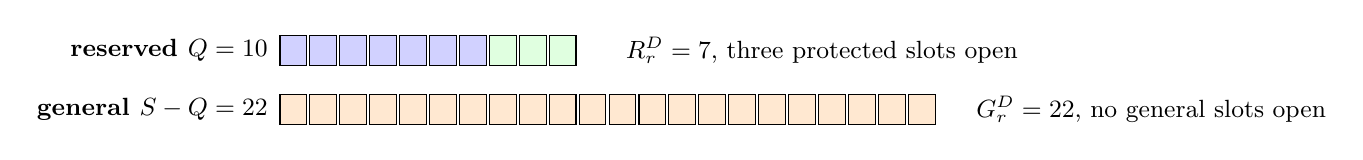
\begin{tikzpicture}[
    every node/.style={font=\small},
    slot/.style={draw, minimum width=0.34cm, minimum height=0.38cm, inner sep=0pt},
    labelnode/.style={font=\small\bfseries}
]
\node[labelnode, anchor=east] at (-0.2,0) {reserved \(Q=10\)};
\foreach \x in {0,...,9} {
    \ifnum\x<7
        \node[slot, fill=blue!18] at (\x*0.38,0) {};
    \else
        \node[slot, fill=green!12] at (\x*0.38,0) {};
    \fi
}
\node[anchor=west] at (4.1,0) {\(R_r^D=7\), three protected slots open};

\node[labelnode, anchor=east] at (-0.2,-0.75) {general \(S-Q=22\)};
\foreach \x in {0,...,21} {
    \node[slot, fill=orange!18] at (\x*0.38,-0.75) {};
}
\node[anchor=west] at (8.55,-0.75) {\(G_r^D=22\), no general slots open};
\end{tikzpicture}
}
\end{center}

Under strict reservation, a Class 1 patient can be offered this day, but a Class 2 patient cannot
use the open protected slots.
\end{examplebox}

\subsection{Residual-Day Search}

\begin{examplebox}[title={Comparing the Earliest Feasible Day}]
Take \(H=4\), \(S=32\), \(Q=10\), and the post-cancellation state below.

\begin{center}
\small
\renewcommand{\arraystretch}{1.45}
\setlength{\tabcolsep}{6pt}
\resizebox{0.98\linewidth}{!}{
\begin{tabular}{|>{\raggedright\arraybackslash}m{2.9cm}|>{\centering\arraybackslash}m{2.1cm}|>{\centering\arraybackslash}m{2.1cm}|>{\centering\arraybackslash}m{2.1cm}|>{\centering\arraybackslash}m{2.1cm}|}
\hline
\rowcolor{gray!15}
\textbf{Count} & \shortstack{\textbf{day \(D\)}\\\(r=0\)} & \shortstack{\textbf{day \(D+1\)}\\\(r=1\)} & \shortstack{\textbf{day \(D+2\)}\\\(r=2\)} & \shortstack{\textbf{day \(D+3\)}\\\(r=3\)} \\
\hline
\cellcolor{gray!10}\(R_r^D\) & \cellcolor{blue!12}\calendarentry{10} & \cellcolor{blue!12}\calendarentry{8} & \cellcolor{blue!12}\calendarentry{10} & \cellcolor{blue!12}\calendarentry{6} \\
\hline
\cellcolor{gray!10}\(G_r^D\) & \cellcolor{orange!18}\calendarentry{22} & \cellcolor{orange!18}\calendarentry{22} & \cellcolor{orange!18}\calendarentry{20} & \cellcolor{orange!18}\calendarentry{13} \\
\hline
\cellcolor{gray!10}\(N_r^D\) & \cellcolor{red!12}\calendarentry{32} & \calendarentry{30} & \calendarentry{30} & \calendarentry{19} \\
\hline
\end{tabular}
}
\normalsize
\end{center}

The implied offers are:
\begin{center}
\small
\begin{tabular}{L{0.26\textwidth} L{0.28\textwidth} L{0.36\textwidth}}
\toprule
\textbf{Policy and class} & \textbf{Earliest offer} & \textbf{Reason} \\
\midrule
Pooled FCFS, either class & \(r=1\) & \(N_1^D=30<32\) \\
\addlinespace
Strict reservation, Class 1 & \(r=1\), reserved & \(R_1^D=8<10\) \\
\addlinespace
Strict reservation, Class 2 & \(r=2\), general & \(G_1^D=22\) is full, but \(G_2^D=20<22\) \\
\bottomrule
\end{tabular}
\normalsize
\end{center}
\end{examplebox}

\section{Daily Simulation Mechanics}

\subsection{Unchanged Daily Order}

The daily event order remains the same as in the v2 note:
\begin{enumerate}[itemsep=0.35em]
    \item \textbf{Compute cancellations for the day.} Future appointments independently cancel with probability \(\phi_i\).
    \item \textbf{Simulate daily arrivals.} \(M_i^D\sim\mathrm{Poisson}(\lambda_i)\).
    \item \textbf{Generate a randomized within-day arrival order.}
    \item \textbf{Apply the configured offer rule.} This is the only step changed by the reserved-slot strategy.
    \item \textbf{Simulate balking.} A class-\(i\) patient offered delay \(\tau\) accepts with probability \(1-b_i(\tau)\).
    \item \textbf{Simulate no-shows and service for day \(D\).}
    \item \textbf{Compute metrics and advance to day \(D+1\).}
\end{enumerate}

\begin{center}
\resizebox{0.98\linewidth}{!}{
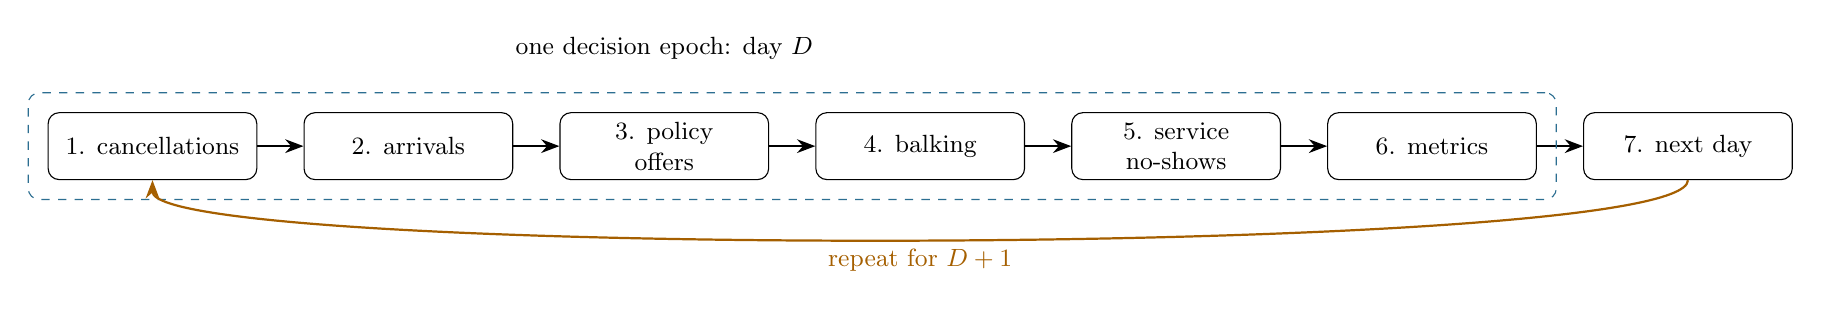
\begin{tikzpicture}[
    >=Stealth,
    every node/.style={font=\small},
    eventstep/.style={draw, rounded corners, align=center, minimum width=2.65cm, minimum height=0.85cm},
    band/.style={draw=FrameBlue, rounded corners, dashed, inner sep=7pt}
]
\node[eventstep] (c) at (0,0) {1. cancellations};
\node[eventstep] (a) at (3.25,0) {2. arrivals};
\node[eventstep] (o) at (6.50,0) {3. policy\\offers};
\node[eventstep] (b) at (9.75,0) {4. balking};
\node[eventstep] (s) at (13.00,0) {5. service\\no-shows};
\node[eventstep] (m) at (16.25,0) {6. metrics};
\node[eventstep] (n) at (19.50,0) {7. next day};

\draw[->, thick] (c) -- (a);
\draw[->, thick] (a) -- (o);
\draw[->, thick] (o) -- (b);
\draw[->, thick] (b) -- (s);
\draw[->, thick] (s) -- (m);
\draw[->, thick] (m) -- (n);
\node[band, fit=(c)(a)(o)(b)(s)(m)] {};
\node[above=0.55cm of o] {one decision epoch: day \(D\)};
\draw[->, thick, FrameGold] (n.south) .. controls +(0,-1.0) and +(0,-1.0) .. node[below] {repeat for \(D+1\)} (c.south);
\end{tikzpicture}
}
\end{center}

\subsection{Strict Reservation Day}

Under strict reservation, the randomized arrival order is processed once. The difference from pooled
FCFS is that the feasible capacity set depends on the patient's class:
\[
\mathcal F_{1,\mathrm{strict}}^D
=
\left\{(r,\mathrm{res}):r\in\mathcal R,\ R_r^D<Q\right\}
\cup
\left\{(r,\mathrm{gen}):r\in\mathcal R,\ G_r^D<S-Q\right\},
\]
where reserved capacity is checked before general capacity on the same residual day. For Class 2,
\[
\mathcal F_{2,\mathrm{strict}}^D
=
\left\{(r,\mathrm{gen}):r\in\mathcal R,\ G_r^D<S-Q\right\}.
\]

If \(\mathcal F_{i,\mathrm{strict}}^D\) is empty, that patient receives no offer. The simulator then
continues to later arrivals because a later Class 1 arrival may still have protected capacity even
when a Class 2 arrival has no general capacity.

\section{Comparison to Pooled FCFS}

\subsection{Policy Effects}

\begin{center}
\small
\resizebox{\linewidth}{!}{
\begin{tabular}{L{0.25\textwidth} L{0.30\textwidth} L{0.35\textwidth}}
\toprule
\textbf{Feature} & \textbf{Pooled FCFS} & \textbf{Strict Class 1 reservation} \\
\midrule
Capacity structure & all \(S\) slots pooled & \(Q\) protected, \(S-Q\) general \\
\addlinespace
Class 1 access & competes only by arrival order & protected first, then general overflow \\
\addlinespace
Class 2 access & can use any open slot & can use only general slots \\
\addlinespace
Unused reserved slots & not applicable & may remain empty \\
\addlinespace
Utilization tendency & highest when demand is sufficient and no-shows are low & can fall if Class 1 demand is not enough to use \(Q\) \\
\addlinespace
Equity/access tendency & neutral in the offer rule; differences come from behavior & shifts access toward Class 1 \\
\bottomrule
\end{tabular}
}
\normalsize
\end{center}

\subsection{Expected Metric Patterns}

The main metrics are unchanged:
\[
\rho^{\mathrm{attended}}
=
\frac{\mathrm{served\ slots}}{S\times\mathrm{measured\ days}},
\qquad
\rho^{\mathrm{booked}}
=
\frac{\mathrm{booked\ slots\ on\ service\ days}}{S\times\mathrm{measured\ days}},
\qquad
\mathrm{served\ rate}_i
=
\frac{\mathrm{served}_i}{\mathrm{arrivals}_i}.
\]
\(\rho^{\mathrm{attended}}\) is completed-visit utilization.  For the reservation analysis,
\(\rho^{\mathrm{booked}}\) is also useful because it shows whether protected slots were actually
occupied on the schedule.  No-shows count as booked slots; appointments that cancel early enough to
free the service-day slot do not.

The reservation strategy mainly affects the path to those metrics:
\[
\text{offer rule}
\rightarrow
\tau
\rightarrow
b_i(\tau)
\rightarrow
\text{booked patients}
\rightarrow
\phi_i,\ \xi_i(\tau)
\rightarrow
\text{served patients}.
\]

\begin{keybox}[title={Interpretation of the Comparison}]
Strict reservation can improve Class 1 access while lowering booked-slot utilization if protected
slots are not filled.  It can also lower attended utilization if booked slots turn into no-shows.
\end{keybox}

\subsection{Objective-Function Analysis}

The metrics above describe what happened in one simulation run. The objective-function analysis
adds one more step: it turns each FCFS run and each strict-reservation run into a single comparable
score. This is useful because strict reservation can improve Class 1 outcomes while also leaving
some protected capacity unused. In this section the main capacity score is booked-slot utilization,
because the policy question is whether protected slots are actually occupied. Completed-visit
utilization remains a related diagnostic for no-show losses. A single metric is therefore not enough
to decide whether a given \(Q\) is attractive.

The objective functions are not a new booking policy. The booking policies remain pooled FCFS and
strict Class 1 reservation. The objective functions are only used after the simulation to compare
the resulting outcomes.

\subsubsection{Policy Parameter}

The main policy parameter is the protected daily capacity
\[
Q=\text{number of Class 1 reserved slots per day}.
\]
In the visual examples above, \(Q=10\) and \(S=32\) are fixed to make the mechanics concrete. In
the objective-function notebooks, \(Q\) is swept across a range of values and compared against the
matched FCFS baseline, where \(Q=0\).

It is helpful to scale the cost of reservation by the protected share of the day:
\[
\frac{Q}{S}.
\]
This treats one protected slot as more expensive when the clinic has fewer total daily slots.

\subsubsection{Initial Analysis Grid}

The first objective-function notebooks center the sweep around the realistic demand scale rather
than the larger visual example in this note. The baseline analysis uses total daily demand
\(\lambda\approx 25\), Class 1 share \(p=0.58\), and daily capacity \(S=20\). The main \(Q\) sweep is
\[
Q\in\{0,1,2,3,4,5,6,8,10,12\}.
\]
Demand and mix are varied around that center:
\[
\lambda\in\{15,20,25,30,35,40,50\},
\qquad
p\in\{0.40,0.50,0.58,0.65,0.75\}.
\]

The initial weight and penalty values are
\[
w_1\in\{1,1.25,1.5,2,3\},
\qquad
c\in\{0,0.02,0.05,0.10\},
\qquad
\gamma\in\{0,0.02,0.05,0.10\},
\]
with \(w_2=1\). The headline setting is \(w_1=1.5\), \(c=0.05\), and
\(\gamma=0.05\). These values are not claimed to be final; they are starting values for finding
which parts of the demand and behavior space make strict reservation look better than FCFS.

\subsubsection{Weighted Booked Slot Use}

For class-specific booked slot use, define each class contribution as
\[
\rho_i^{\mathrm{booked}}
=
\frac{\mathrm{served}_i+\mathrm{no\ show}_i}{S\times\mathrm{measured\ days}}.
\]

The weighted booked-slot objective is
\[
U_{\mathrm{booked}}(w_1,w_2)
=
w_1\rho_1^{\mathrm{booked}}
+
w_2\rho_2^{\mathrm{booked}}.
\]
Class 2 is kept at \(w_2=1\). Increasing \(w_1\) makes Class 1 booked slots count more in the
comparison. When \(w_1=w_2=1\), this reduces to total booked-slot utilization
\(\rho^{\mathrm{booked}}\).

The completed-visit version is still available as a diagnostic:
\[
\rho_i^{\mathrm{attended}}
=
\frac{\mathrm{served}_i}{S\times\mathrm{measured\ days}}.
\]
This separates empty protected slots from booked slots that later no-show.

\subsubsection{Weighted Served Rate}

The class served-rate metric from the previous subsection is
\[
\mathrm{served\ rate}_i
=
\frac{\mathrm{served}_i}{\mathrm{arrivals}_i}.
\]

The weighted served-rate objective compares weighted served patients to weighted arrivals:
\[
U_{\mathrm{served}}(w_1,w_2)
=
\frac{
w_1\mathrm{served}_1+w_2\mathrm{served}_2
}{
w_1\mathrm{arrivals}_1+w_2\mathrm{arrivals}_2
}.
\]
This objective is bounded between 0 and 1 before any penalty is applied. It answers a direct
access question: after giving Class 1 a higher weight, what share of weighted demand was served?

\subsubsection{Slot-Cost Penalty}

Strict reservation protects access, but protected slots can be left empty if Class 1 demand is not
large enough or if Class 1 behavior leads to cancellations, no-shows, or balking. To reflect that
tradeoff, the net booked-slot objective subtracts a cost for configured protected capacity:
\[
U_{\mathrm{net\ booked}}(w_1,w_2,c)
=
U_{\mathrm{booked}}(w_1,w_2)
-
c\frac{Q}{S}.
\]
Here \(c\) controls how expensive protected capacity is. A larger \(c\) makes high-\(Q\) policies
harder to justify unless they create enough weighted booked-slot benefit.  The notebooks also keep
the served-rate version \(U_{\mathrm{served}}(w_1,w_2)-cQ/S\) as an access diagnostic.

\subsubsection{Waiting-Time Penalty}

Because the simulator stores the originally offered delay \(\tau\), a waiting-time version can also
be evaluated. For offered patients, define the weighted average offered delay
\[
\bar{\tau}_w
=
\frac{
w_1\sum_{\mathrm{offered\ class\ 1}}\tau
+
w_2\sum_{\mathrm{offered\ class\ 2}}\tau
}{
w_1\mathrm{offered}_1+w_2\mathrm{offered}_2
}.
\]

The wait-adjusted objective is
\[
U_{\mathrm{wait}}(w_1,w_2,c,\gamma)
=
U_{\mathrm{booked}}(w_1,w_2)
-
c\frac{Q}{S}
-
\gamma\frac{\bar{\tau}_w}{H}.
\]
The term \(\bar{\tau}_w/H\) normalizes offered delay by the booking horizon. The parameter
\(\gamma\) controls how strongly longer offered waits should lower the score.

\subsubsection{Basic Requirements}

Some comparisons are easier to read as a requirements check rather than a single score. The
notebooks therefore also record whether a run satisfies
\[
\rho^{\mathrm{booked}}\ge \rho_{\min},
\qquad
\min_i\ \mathrm{served\ rate}_i\ge x,
\qquad
\left|\rho_1^{\mathrm{booked}}-\rho_2^{\mathrm{booked}}\right|\le g.
\]
Here \(\rho_{\min}\) is the minimum booked-slot utilization level, \(x\) is the minimum served-rate
floor for each class, and \(g\) is the largest allowed gap between the two class-specific booked-slot
utilization contributions.

\subsubsection{Matched Comparison to FCFS}

Each strict-reservation run is compared to a pooled FCFS run with the same scenario and seed. For a
scenario \(a\), seed \(j\), and objective \(U\), the paired difference is
\[
\Delta U(Q;a,j)
=
U_{\mathrm{strict}}(Q;a,j)
-
U_{\mathrm{FCFS}}(a,j).
\]
The sweep averages this paired difference over \(J\) seeds:
\[
\overline{\Delta U}(Q)
=
\frac{1}{J}\sum_{j=1}^{J}\Delta U(Q;a,j).
\]
The best protected capacity for a scenario is the \(Q\) with the highest average paired difference:
\[
Q^\star(a)
=
\operatorname*{arg\,max}_{Q}\ \overline{\Delta U}(Q;a).
\]

The notebooks label a setting as a clear win when the average paired difference is positive and the
lower end of the 95 percent interval is also positive. If the average is positive but the interval
crosses zero, the setting is a possible win. Otherwise it is treated as a loss relative to FCFS.

\begin{keybox}[title={How to Read the Objective Analysis}]
The goal is not to find one universal \(Q\). The goal is to find when strict reservation beats FCFS
for a stated priority weight, a stated cost of protected capacity, and a stated demand and behavior
scenario.
\end{keybox}

\subsection{No-Offer Interpretation}

The no-offer event has a slightly different meaning across the strategies:
\begin{center}
\small
\begin{tabular}{L{0.25\textwidth} L{0.65\textwidth}}
\toprule
\textbf{Policy} & \textbf{No-offer meaning} \\
\midrule
Pooled FCFS & no day in \(\mathcal R\) satisfies \(N_r^D<S\) \\
\addlinespace
Strict reservation, Class 1 & no day has either \(R_r^D<Q\) or \(G_r^D<S-Q\) \\
\addlinespace
Strict reservation, Class 2 & no day has \(G_r^D<S-Q\), even if \(R_r^D<Q\) somewhere \\
\bottomrule
\end{tabular}
\normalsize
\end{center}

\section{Implementation Mapping}

\subsection{Config Objects}

The new implementation fields map directly to the notation:
\begin{center}
\small
\begin{tabular}{L{0.30\textwidth} L{0.22\textwidth} L{0.36\textwidth}}
\toprule
\textbf{Code field} & \textbf{Notation} & \textbf{Meaning} \\
\midrule
\texttt{slots\_per\_day} & \(S\) & total daily capacity \\
\addlinespace
\texttt{reserved\_class\_id} & \(i^\star\) & protected class; here \(i^\star=1\) \\
\addlinespace
\texttt{reserved\_slots\_per\_day} & \(Q\) & protected daily capacity; here \(Q=10\) \\
\addlinespace
\texttt{Booking.reserved\_slot} & pool label \(z\) & true means the appointment was placed in the reserved pool \\
\bottomrule
\end{tabular}
\normalsize
\end{center}

\subsection{Code Path}

The policy logic appears in the booking step:
\begin{itemize}[nosep]
    \item \texttt{find\_earliest\_open\_day} computes the earliest feasible \((r,z)\) pair.
    \item \texttt{process\_daily\_arrivals} applies the one-pass arrival order.
    \item For Class 1, \texttt{find\_earliest\_open\_day} searches each residual day as reserved then general.
    \item For Class 2, \texttt{find\_earliest\_open\_day} searches general capacity only.
\end{itemize}

\begin{reviewbox}[title={Review Against the Implemented Reserved-Slot Model}]
\begin{itemize}[nosep]
    \item The original day-level state notation \(X_{i,r}^{D}\), \(N_r^D\), \(r\), \(\tau\), \(S\), and \(H\) is unchanged.
    \item The new audit-layer pool counts \(R_r^D\) and \(G_r^D\) split the same daily capacity into reserved and general pools.
    \item \(Q=10\) protected slots are reserved for Class 1 out of \(S=32\).
    \item In strict reservation, unused protected slots stay unavailable to Class 2.
    \item Cancellation, no-show, service, and metric definitions remain the same as in the FCFS v2 note.
\end{itemize}
\end{reviewbox}

\section{Conclusion}

The reservation strategy is not a separate patient behavior model. It is a change to the offer
rule inside the same day-level appointment simulator. Pooled FCFS uses one capacity constraint
\[
N_r^D<S.
\]
Strict Class 1 reservation replaces that with class-dependent eligibility over
\[
R_r^D<Q
\qquad\text{and}\qquad
G_r^D<S-Q.
\]

The comparison should therefore be read as an access/utilization tradeoff:
\[
\text{more Class 1 protection}
\quad\Longleftrightarrow\quad
\text{less automatic pooling of daily capacity}.
\]

\end{document}
